\chapter{Metriche}

In questo capitolo verranno descritte le metriche anticipate nella Sezione
\ref{descrizione_progetto}, mostrando il relativo codice e i risultati ottenuti.

\section{Metriche sulle conferenze}

Questa sezione tratta delle varie metriche relative all'insieme di conferenze
analizzate, che conta un totale di più di 500 conferenze.

\subsection{Rating delle conferenze}

Come descritto in Sezione~\ref{sec:conferenze}, le conferenze possono avere
un rating, rappresentato da una lettera, che rappresenta la qualità generale
della conferenza.

Al fine di comprendere al meglio come questa classifica influenza i vari indici
bibliometrici, in Figura~\ref{fig:conferences-distribution} viene rappresentata
la suddivisione delle conferenze in base alla loro qualità come classificata
dal GGS.

\begin{figure}[tb]
  \centering
  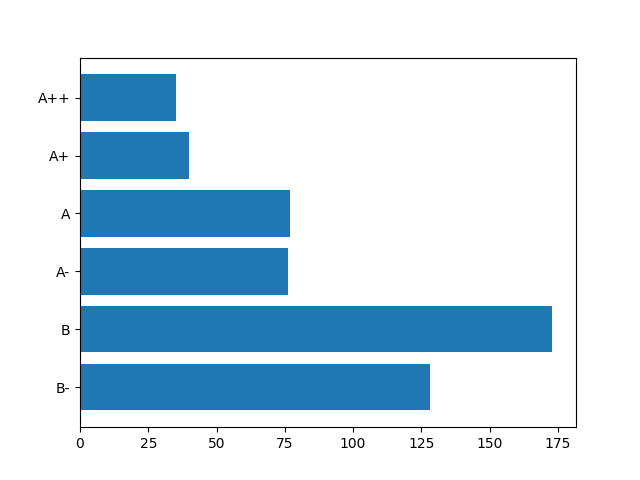
\includegraphics[width=\linewidth]{conferences-distribution.png}
  \caption{Distribuzione delle conferenze}
  \label{fig:conferences-distribution}
\end{figure}

È immediato notare che la distribuzione è suddivisa in 3 gruppi principali:
\begin{enumerate}
  \item Il gruppo delle ``conferenze top'', dato dalle A++ e dalle A+, che
        risulta essere il più contenuto di tutti con meno di 100 conferenze;
  \item Il secondo gruppo delle conferenze di alto livello, dato dalle A e A-,
        che risulta comunque non molto più grande del precedente con circa 150
        conferenze;
  \item Ed infine il gruppo delle conferenze B e B-, che domina in quanto a numero
        i precedenti due, avendo più conferenze degli altri due gruppi combinati.
\end{enumerate}

Questo conferma quello che ci si può aspettare con la classificazione per qualità in molti ambiti: in generale, la qualità alta è correlata
con una numerosità minore.

Ciò fa sì che conferenze con qualità più alta, essendo in numero minore,
ricevano una competizione maggiore rispetto a quelle di qualità più bassa, in
quanto una conferenza di ottimo livello tenderà ad essere più critica sui lavori
ricevuti al fine di mantenere tale ranking. D'altra parte, una conferenza con
ranking minore potrebbe puntare maggiormente sulla quantità di paper al fine di
crescere di dimensioni per poter avere una possibilità di salire di ranking,
ma a scapito del controllo della qualità dei lavori ad essa sottomessi. Questo infatti è uno dei criteri considerati dal CORE per la valutazione della qualità di una conferenza (come approfondito nella Sezione \ref{sec:conferenze_scientifiche}).

\subsection{Numero di citazioni per paper in base al rating}

Si vuole ora guardare a come la qualità di una conferenza influenza il numero
di citazioni che un paper prende in media. Il numero di citazioni di un paper
è una metrica importante per un ricercatore, in quanto è uno dei fattori
che contribuisce ai suoi indici principali, tra cui l'$h$-index.

La Figura~\ref{fig:paper-rating-distribution} mostra appunto tale distribuzione,
rappresentando con un punto il numero di citazioni di ogni singolo paper e
con una linea rossa la media di citazioni in base al rating della conferenza
a cui il paper è stato sottomesso. I valori di tale media sono visibili
anche in Tabella~\ref{table:paper-rating-distribution}.

\begin{figure}[tb]
  \centering
  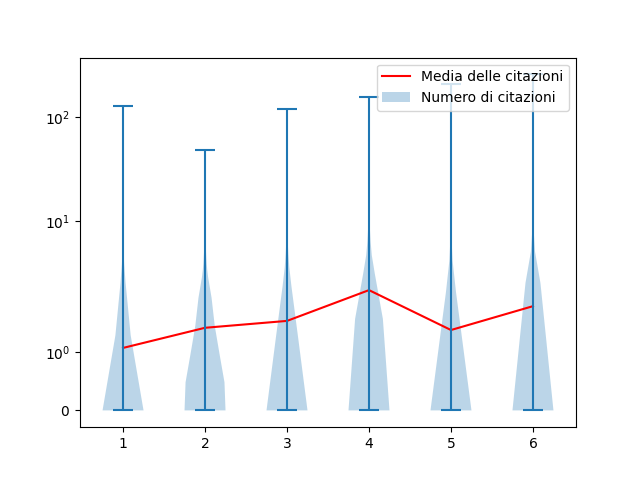
\includegraphics[width=\linewidth]{paper_rating_distribution.png}
  \caption{Numero di citazioni per conferenza}
  \label{fig:paper-rating-distribution}
\end{figure}

\begin{figure}[tb]
  \centering
  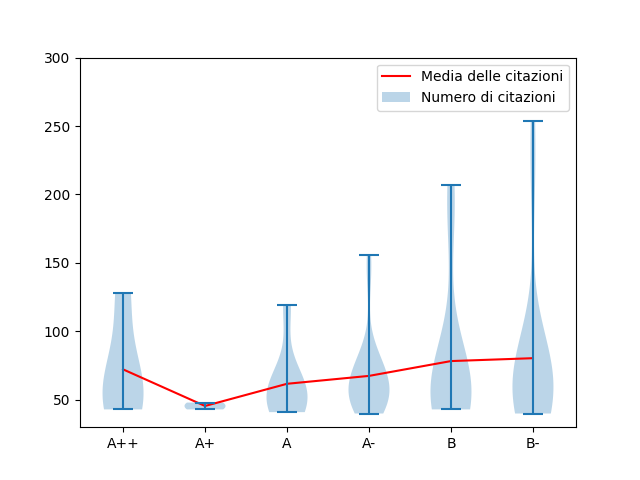
\includegraphics[width=\linewidth]{paper_rating_distribution_impact.png}
  \caption{Numero di citazioni di paper di impatto per conferenza}
  \label{fig:paper-rating-distribution-impact}
\end{figure}

\begin{table}[tb]
  \centering
  \begin{tabular}{||l | r | r ||}
    \hline
    \multirow{2}{*}{\textbf{Rating}} & \multicolumn{2}{| c ||}{\textbf{Numero di citazioni medio}} \\ \cline{2-3}
     & \textbf{Tutti i paper} & \textbf{Paper di impatto} \\ [0.5ex] 
    \hline\hline
    A++    & 1.08 & 72.25 \\ \hline
    A+     & 1.42 & 45.50 \\ \hline
    A      & 1.54 & 61.71 \\ \hline
    A-     & 2.19 & 67.48 \\ \hline
    B      & 1.38 & 78.32 \\ \hline
    B-     & 1.80 & 80.41 \\ \hline
  \end{tabular}
  \caption{Numero di citazioni medio per rating}
  \label{table:paper-rating-distribution}
\end{table}

Dall'immagine è possibile trarre due conclusioni importanti:
\begin{enumerate}
  \item La prima è che, in media, le citazioni per un paper sono basse sul
        periodo di qualche anno che è stato considerato;
  \item La seconda, invece, è che la distribuzione delle citazioni è molto sbilanciata,
        in quanto ci sono molti paper con poche citazioni e pochi paper che superano
        le 40 citazioni.
\end{enumerate}

Queste due conclusioni valgono inoltre per qualsiasi ranking di conferenza,
con un leggero aumento per le conferenze di livello inferiore.
Si può quindi dedurre che, in genere, il livello di una conferenza non influenza
il numero di citazioni ottenute nel breve periodo, con anzi
un aumento delle citazioni in media per conferenze non top, ovvero con ranking
da A in giù.

Può essere interessante inoltre guardare ai paper che possiamo definire come
``d'impatto'', ovvero i pochi paper che superano le 40 citazioni identificati
dalle conclusioni precedenti. Tale distribuzione è visibile in
Figura~\ref{fig:paper-rating-distribution-impact} e, similmente a prima,
è possibile vedere i numeri precisi in
Tabella~\ref{table:paper-rating-distribution}.
Guardando il grafico, è possibile notare che i paper con citazioni più alte
si trovano sulle conferenze di rating più basso, ma questi risultano essere più
valori rari che si discostano molto dalla media. Sulle conferenze di livello
più alto, invece, la distribuzione è molto meno sbilanciata: i paper sono più
concentrati sotto le 150 citazioni, ma in genere la distribuzione di citazioni
è più equa. Questo si vede chiaramente per le conferenze A++.

\subsection{Media dell'$h$-index per conferenza in base al rating}

Oltre al numero di citazioni, è interessante guardare anche
a come l'$h$-index degli autori è correlato con il rating delle conferenze
a cui partecipano. Questo perché ci si aspetta che conferenze con un rating
maggiore attirino ricercatori con più esperienza, in quanto il loro
processo di accettazione è sicuramente più selettivo rispetto a conferenze
più nuove oppure semplicemente classificate come di livello inferiore.

Nella Figura~\ref{fig:h-index-vs-rating} si vede appunto questa metrica,
rappresentata tramite un grafico a violino con in rosso la media dell'$h$-index
per rating della conferenza, i cui valori precisi sono visibili in
Tabella~\ref{table:h-index-vs-rating}.

\begin{figure}[tb]
  \centering
  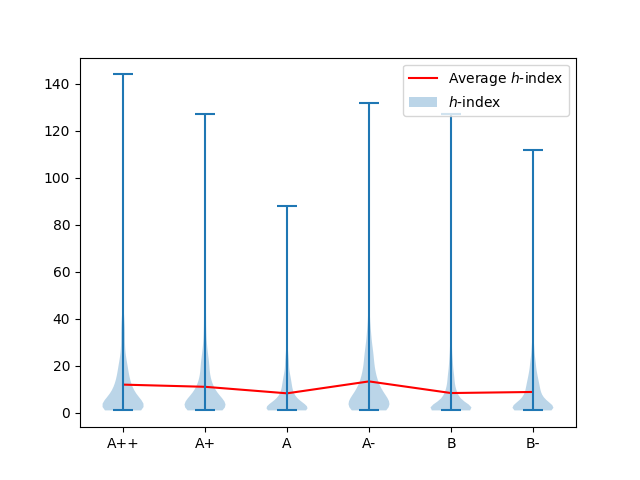
\includegraphics[width=\linewidth]{h_index_vs_conference_rating.png}
  \caption{$h$-index per conferenza}
  \label{fig:h-index-vs-rating}
\end{figure}

\begin{table}[tb]
  \centering
  \begin{tabular}{||l|r||}
    \hline
    \textbf{Rating conferenza} & \textbf{$h$-index medio} \\ [0.5ex] 
    \hline\hline
    A++    & 11.97 \\ \hline
    A+     & 11.04 \\ \hline
    A      & 8.27  \\ \hline
    A-     & 13.34 \\ \hline
    B      & 8.39 \\ \hline
    B-     & 8.84 \\ \hline
  \end{tabular}
  \caption{Valori medi dell'$h$-index}
  \label{table:h-index-vs-rating}
\end{table}

Come si può vedere dai dati, per le conferenze di livello ottimo (A++ e A+)
si ha un $h$-index maggiore in media, pari a circa $11.51$, rispetto a quelle
degli altri due livelli ($10.81$ per le conferenze A e A-, $8.62$ per le B e
B-).

Questo coincide con le aspettative: conferenze di livello maggiore hanno
un processo selettivo più restrittivo e di conseguenza è più probabile
che un ricercatore con più esperienza (e quindi con $h$-index probabilmente
più alto) sottoponga lavori a queste conferenze.

Notare comunque che la differenza fra le varie categorie non è così elevata,
e le curve sono fortemente sbilanciate verso $h$-index bassi in ogni caso,
anche se ciò è più visibile nelle conferenze di rating B e B-.

\section{Metriche sulle affiliazioni}

Questa sezione tratta di alcune metriche per le affiliazioni, in particolare
raggruppate per stato di appartenenza. Ciò al fine di capire al meglio
in che aree e in che realtà si concentra la ricerca in ambito informatico.

Il numero di affiliazioni considerate conta poco meno di 13000 fra università
e centri di ricerca, con un totale di 131 nazioni.

\subsection{Autori e documenti per stato di appartenenza}
\label{ssec:authors-docs-per-country}

Tale metrica viene analizzata principalmente come base per le successive, in
quanto uno stato con molti più autori ha anche molta più probabilità di avere
università considerate migliori, il che potrebbe portare ad un aumento
in generale dell'$h$-index medio o della qualità della ricerca.
Tale numero è visibile, per le prime 10 nazioni in ordine di numero di autori,
in Figura~\ref{fig:num-authors-per-country}.

Inoltre, sono stati anche calcolati il numero di documenti prodotti dalle singole
nazioni, per ragioni simili a quelle esplicate nel paragrafo precedente: un
paese con molti più documenti rappresenta una maggiore concentrazione della
ricerca, che potrebbe essere correlata con maggiore qualità.
Tale metrica è visibile in Figura~\ref{fig:num-documents-per-country}.

\begin{figure}[tb]
  \centering
  \begin{subfigure}[b]{0.45\textwidth}
    \centering
    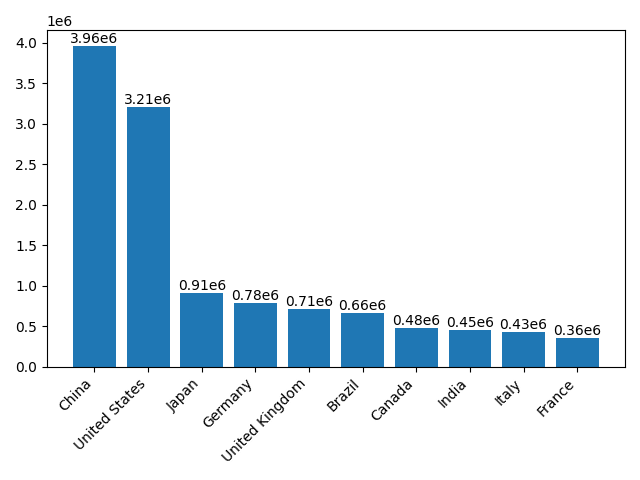
\includegraphics[width=\textwidth]{num_authors_per_country.png}
    \caption{Numero di autori}
    \label{fig:num-authors-per-country}
  \end{subfigure}
  \begin{subfigure}[b]{0.45\textwidth}
    \centering
    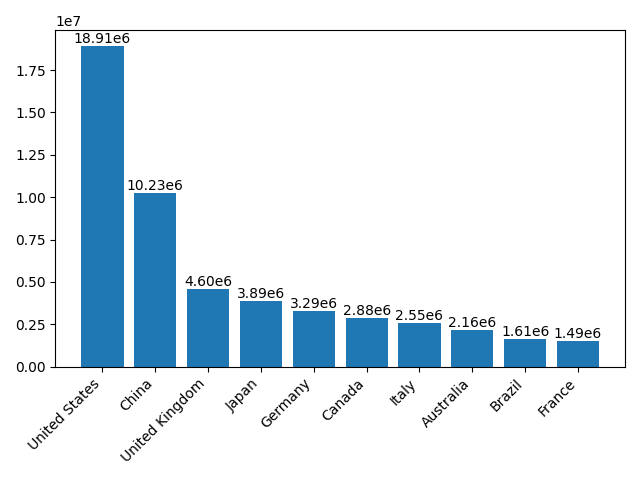
\includegraphics[width=\textwidth]{num_documents_per_country.png}
    \caption{Numero di documenti}
    \label{fig:num-documents-per-country}
  \end{subfigure}
  \caption{Primi 10 stati secondo varie metriche}
  \label{fig:top-10-country}
\end{figure}

Non sorprendentemente, i dati raccolti confermano che gli attuali stati
con più ricercatori in ambito di computer science sono la Cina e gli Stati Uniti,
dopo i quali il numero di autori diventa meno di un terzo per altri paesi
dell'Asia, dell'Europa e del Nord America.
Per quanto riguarda i documenti, invece, gli Stati Uniti dominano, ma sono
seguiti a breve distanza dalla Cina.

Di conseguenza, ci si aspetta che la Cina e gli Stati Uniti tengano delle buone
posizioni nelle successive classifiche, in quanto dispongono di un parco maggiore
di ricercatori e producono un maggiore numero di documenti.

Interessante notare l'Italia che si pone come terza nazione europea per numero
di autori, dietro a Germania e Regno Unito, in entrambi i casi.

\subsection{Maggiori entità per produttività}

In genere guardare al solo numero assoluto di autori o documenti di un certo
stato è sì interessante, ma lontano dal quadro completo. Per questo si è
deciso di introdurre un'ulteriore metrica, qui chiamata \textit{produttività},
definita semplicemente come il rapporto fra il numero di documenti ed il
numero di autori. In tal modo, un valore alto di produttività indica uno
stato in cui i ricercatori producono in media più lavori rispetto ad un
altro. Nella Figura~\ref{fig:productivity-per-country} vengono quindi mostrati i valori
di produttività calcolati sugli stati con maggiore numero di autori e di
documenti, ovvero gli stati visibili in Figura~\ref{fig:top-10-country} alla
Sezione~\ref{ssec:authors-docs-per-country}.

\begin{figure}[tb]
  \centering
  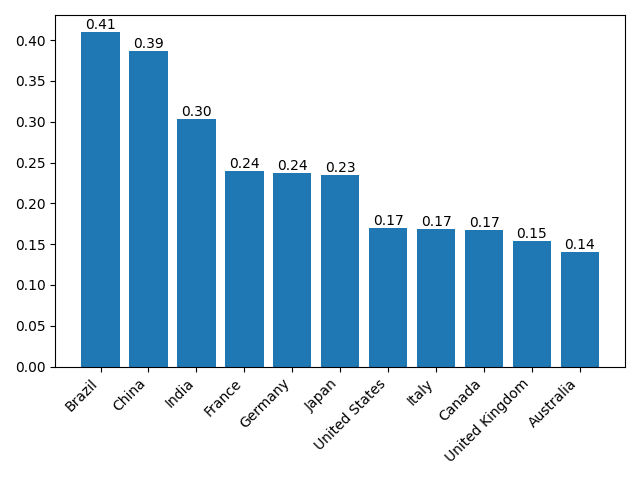
\includegraphics[width=\linewidth]{productivity_per_country.png}
  \caption{Produttività per le maggiori nazioni}
  \label{fig:productivity-per-country}
\end{figure}

Dalla figura compare uno scenario leggermente diverso: le maggiori nazioni
per produttività non sono le maggiori per numero di documenti o autori, eccezion
fatta per la Cina. La produttività maggiore va invece verso nazioni come Brasile
e India, subito seguite da Francia e Germania.
Di conseguenza, i paesi in cui i ricercatori producono più lavori in media
sono i paesi cosiddetti ``emergenti''.


\section{Metriche sugli autori}

In questa sezione ci si vuole concentrare maggiormente su come metriche e
indici relativi ai singoli autori dipendono da altri fattori, quali la
dimensione dell'affiliazione con cui pubblicano.

In particolare, sono state prese in considerazione metriche \textit{aggregate},
in quanto possono dare una visione d'insieme su quello che sarebbe un numero
troppo elevato di autore da poter analizzare singolarmente.

\subsection{Correlazione fra numero di citazioni e dimensione dell'affiliazione}
\label{ssec:correlazione-citazioni-dimensione-affiliazione}

Con questa analisi si guarda ad una possibile correlazione fra il numero di
citazioni totale di un autore e la dimensione della sua affiliazione, in
quanto a numero di autori.
Così facendo, è possibile capire se un'università con molto personale
può risultare vantaggiosa quando si tratta di far conoscere i lavori pubblicati
da un ricercatore, senza però far variare necessariamente l'$h$-index (questo
sarà guardato in Sezione~\ref{ssec:correlazione-h-index-dimensione-affiliazione}).
È sì possibile che in generale un numero alto di citazioni può portare anche ad
un elevato $h$-index, ma non è necessariamente sempre vero: con questa analisi
si vuole capire semplicemente quanto i lavori di un certo autore sono conosciuti,
senza guardare forzatamente a quanto tale autore è considerato buono o meno
dal punto di vista dell'$h$-index.

Al fine di evitare una quantità troppo elevata di informazioni, le affiliazioni
sono state divise in vari \textit{bucket} rispetto alla loro dimensione, che
di specifico sono:
\begin{itemize}
  \item Affiliazioni molto piccole (meno di 10 autori) e piccole (fra 10 e
        100 autori) che possono rappresentare, per esempio, centri di ricerca
        aziendali o molto specifici;
  \item Affiliazioni di buona dimensione, fra 100 e 1000 autori, in cui
        ricadono molte università;
  \item Affiliazioni grandi, fra 1000 e 10000 autori;
  \item Affiliazioni molto grandi, oltre i 10000 autori.
\end{itemize}
%
Inoltre, sempre per poter rappresentare graficamente al meglio informazioni
utili, sono stati esclusi gli \textit{outlier} da tale distribuzione, in quanto
sono pochissimi casi con valori molto alti che non contribuiscono molto però
alla distribuzione nel suo insieme.

\begin{figure}[tb]
  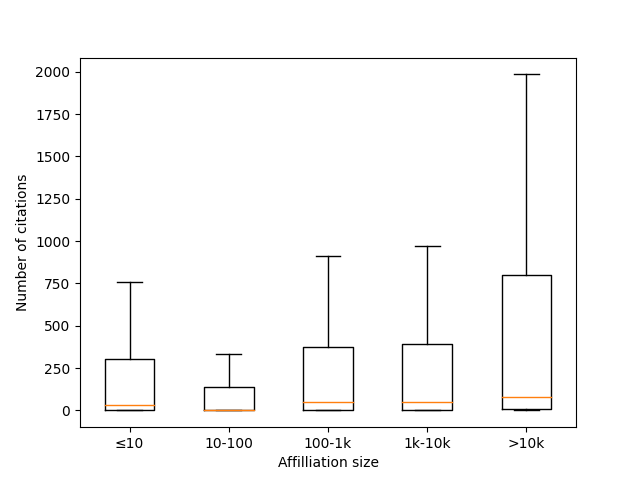
\includegraphics[width=\linewidth]{author_citations_vs_affiliation_size}
  \caption{Relazione fra citazioni e dimensione dell'affiliazione}
  \label{fig:author-citations-vs-affiliation-size}
\end{figure}

Come si può vedere dalla Figura~\ref{fig:author-citations-vs-affiliation-size},
per le affiliazioni con dimensioni sotto i 10000 autori non c'è molta differenza,
sebbene si ha una leggera crescita delle code della distribuzione con la crescita
della dimensione dell'affiliazione.
La differenza sostanziale si vede quando l'affiliazione supera i 10000 autori:
in tal caso, sia la maggior parte degli autori sia la coda della distribuzione
ricevon più citazioni in media di ricercatori affiliati ad entità di dimensioni
inferiori.
Di conseguenza, si può dedurre che la dimensione dell'affiliazione con cui
si decide di pubblicare conta solo se essa è molto grande, ma in modo comunque
non eccessivo, visto che la media (rappresentata dalla riga orizzontale
arancione) rimane paragonabile in tutti i casi.

\subsection{Correlazione fra $h$-index e dimensione dell'affiliazione}
\label{ssec:correlazione-h-index-dimensione-affiliazione}

Similmente alla Sezione~\ref{ssec:correlazione-citazioni-dimensione-affiliazione},
in questa sezione si vuole guardare invece ad una possibile correlazione fra la
dimensione dell'affiliazione di un autore e il valore del suo $h$-index.
A differenza del puro numero di citazioni, l'$h$-index dipende anche dalla
quantità di paper scritti da un certo autore, e quindi non è semplicemente una
misura della ``popolarità'' del suo lavoro di ricerca, ma è più vicina ad una
misura pesata fra quantità e qualità dei lavori.

Per questa analisi valgono le stesse considerazioni esposte in
Sezione~\ref{ssec:correlazione-citazioni-dimensione-affiliazione}: le affiliazioni
sono state separate in vari gruppi in base al numero di autori (meno di 10, fra
10 e 100, fra 100 e 1000, fra 1000 e 10000, e più di 10000), ed anche per questa
analisi non sono rappresentati gli \textit{outlier}.

\begin{figure}[tb]
  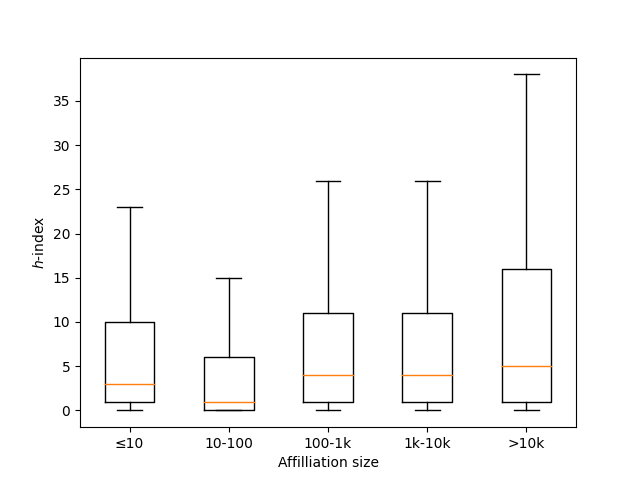
\includegraphics[width=\linewidth]{author_h_index_vs_affiliation_size}
  \caption{Relazione fra $h$-index e dimensione dell'affiliazione}
  \label{fig:author-h-index-vs-affiliation-size}
\end{figure}

I risultati visibili in Figura~\ref{fig:author-h-index-vs-affiliation-size}
sono paragonabili, in quanto a forma, a quelli visti in
Sezione~\ref{ssec:correlazione-citazioni-dimensione-affiliazione},
Figura~\ref{fig:author-citations-vs-affiliation-size}.
Per le affiliazioni di dimensioni non considerevoli (i.e., sotto i 10000 autori)
non c'è molta differenza per quanto riguarda l'$h$-index, mentre per le entità
molto grosse allora la distribuzione si sposta di più verso valori alti di
$h$-index, soprattutto per quanto riguarda le code della distribuzione.
Similmente a prima, la media resta paragonabile, anche se con leggera crescita
in base alla dimensione dell'affiliazione.


%%metriche su principali conferenze
\section{Metriche sulle principali conferenze}
In aggiunta alle metriche presentate finora, si è voluto fare un confronto più ristretto, concentrando le analisi sulle principali conferenze che riguardano la sicurezza informatica.

Tali conferenze sono di norma considerate essere CCS, S\&P, USENIX e NDSS. Di queste, nelle analisi sono state considerate solo le prime due in quanto quelle con il maggior numero di dati presenti su Scopus. Inoltre, è dovere delle conferenze inviare i propri \textit{proceedings} a Scopus e non tutte decidono di condividere i propri dati.

La \textit{ACM Conference on Computer and Communications Security}, CCS, è una conferenza che si tiene annualmente dal 1993 e che interessa ricercatori e professionisti che si occupano di sicurezza informatica. È la conferenza di maggior rilievo del SIGSAC (\textit{Special Interest Group on Security, Audit and Control}), la cui missione è quella di sviluppare sempre di più la sicurezza informatica, sponsorizzando conferenze di alta qualità in cui vengono affrontati aspetti riguaranti applicazioni sicure, crittografia, autenticazione, controllo degli accessi, analisi dei rischi e, in generale, tutto ciò che riguarda i sistemi sicuri. Inoltre si analizza la sicurezza nei database, nelle reti e nei sistemi operativi, considderando anche tutte le aree di applicazione che, per esempio, possono essere: la protezione della proprietà intellettuale, la moneta e il commercio elettronico, i sistemi di telecomunicazione. 

L'\textit{IEEE Symposium on Security and Privacy}, S\&P, si occupa, dal 1980, di raccogliere e presentare gli sviluppi riguardanti la security e la privacy. Vengono raccolti articoli che trattano progressi sia a livello teorico che di implementazione. Dal 2016 si è anche organizzato un simposio a livello europeo.

USENIX è un'orgnizzazione no-profit che dal 1975 sostiene e promuove la ricerca sui sistemi informatici avanzati e le conferenze richiamano ingegneri e ricercatori per presentare i loro elaborati riguardanti tutti gli aspetti dei sistemi informatici. Il suo obiettivo è quello di promuovere l'eccellenza e l'innovazione tecnica e la diffusione dell'informatica, fornendo gratuitamente dal 2008 gli atti delle conferenze e le registrazioni degli eventi, attuando una politica dell'\textit{open access}. 

Anche il simposio NDSS (\textit{Network and Distributed System Security}) si occupa, dal 1993, dell'interazione e lo scambio di informazioni sulla sicurezza informatica, concentrandosi prevalentemente su progettazione e implementazione dei sistemi distribuiti. Ogni simposio mette a disposizione indicativamente 120 posti per presentare il proprio progetto di ricerca. Al fine di rendere fruibili le informazioni, i documenti accettati vengono poi messi a disposizione in modo gratuito al termine dell'evento.

\subsection{Distribuzione dell'$h$-index per conferenza}

Confrontando il grafico mostrato in Figura~\ref{fig:h_index_vs_top_conferences} con quello mostrato in Figura~\ref{fig:h-index-vs-rating} si nota che gli $h$-index più bassi dominano rispetto agli altri in entrambi i casi. La differenza è visibile nella presenza maggiore di $h$-index più alti, in particolare attorno a 40.
Questo è atteso in quanto è ragionevole supporre che ricercatori con un profilo di maggior livello, e quindi $h$-index più alto, tendano a sottomettere i loro lavori a conferenze considerate le migliori nel loro campo.

\begin{figure}[tb]
  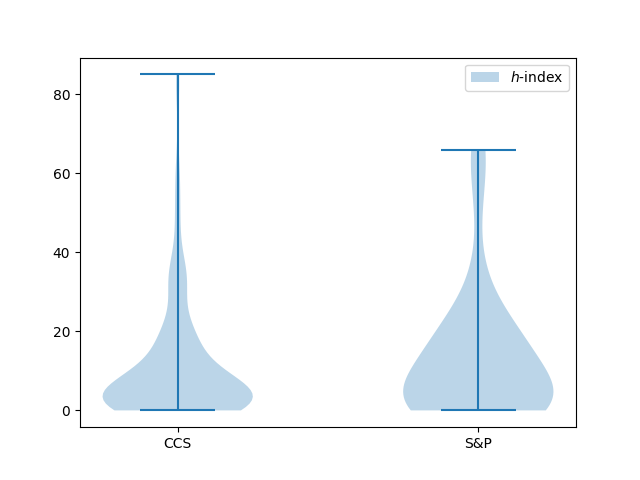
\includegraphics[width=\linewidth]{h_index_vs_top_conferences}
  \caption{Distribuzione di $h$-index per conferenze top}
  \label{fig:h_index_vs_top_conferences}
\end{figure}